\section{Auswertung}
\label{sec:Auswertung}

Die Eckdaten des Geräts lauten 
\begin{align*}
  R_1 = (67,2 \pm 0,1) \mathrm{\Omega} \\
  R_2 = (682 \pm 0,5) \mathrm{\Omega} \\
  L = (16,87 \pm 0,05) \cdot 10^{-3}\mathrm{H} \\
  C = (2,060 \pm 0,003) \cdot 10^{-9}\mathrm{F}.   % ------- 10^-9 oder doch 10^-3? es passt besser -9 weil sonst R_ap komisch wäre 
\end{align*}


Somit ergeben sich die Theoriewerte 
\begin{align*}
  k_{theo} = \frac{R}{2 \cdot L} = 1991,70 \mu \mathrm{(s)^{-1}} \\
  T_{ex} = \frac{R}{4 \pi \cdot L} = 316,99 \mu s\mathrm{\mu s} \\  % evtl nochb R_eff ergänzen? keine formel gefunden
\end{align*}


\subsection{Fehlerformeln}
\label{subsec:fehler}

Bei folgenden Berechnungen werden Mittelwerte mit
\begin{center}
  \begin{equation}
    \mu = \dfrac{1}{N}\sum\limits_{\mathclap{n=1}}^{N}x_n
  \end{equation}
\end{center}

bestimmt. \\
Die Abweichung des Mittelwertes kann dann durch
\begin{center}
  \begin{equation}
    \sigma=\sqrt{\dfrac{1}{N(N-1)}\sum\limits_{n=1}^{N} (x_n - \mu)^2}
  \end{equation}
\end{center}
ermittelt werden. \\
Die Gauß'sche Fehlerfortpflanzung
\begin{center}
  \begin{equation}
    \Delta f = \sqrt{\sum_{i=1}^{N}\left(\partial_{x_i}f\right)^2\cdot{\Delta x_i}^2}
  \end{equation}
\end{center}
kann verwendet werden, wenn fehlerhafte Größen in Rechnungen weiterverwendet werden und dadurch eine neue Abweichung
berechnet werden muss.




\subsection{Berechnung von Abklingdauer und des eff. Dämpfungswiderstandes}
\label{subsec:Abklingdauer und R_daempf}

Die Abklingdauer $T_{ex}$ und der effektive Dämpfungswiderstand $R_{eff}$ können anhand der Zeitabhängigkeit der Kondensatorspannungsamplitude 
bestimmt werden.\\

Der theoretische Verlauf der Kurve lässt sich mit $u_0 = 4V$ durch 
\begin{equation*}
    u(t) = 4 \cdot e^{-\frac{R}{2 \cdot L \cdot t}} = 4 \cdot e^{- 1,99 \cdot 10^{-3} \cdot t}
\end{equation*}
berechnen.\\
Hier wird der Widerstand $R_1$ genutzt. 

\begin{figure}[H]
  \centering
  \includegraphics[scale=0.07]{content/v354a2.png}
  \caption{Die gemessene Kondensatorspannung im RLC-Kreis bei anliegender Rechteckspannung. Zeit t in $20\mu s/Div$ und U in $0.2V/Div$.}
  \label{fig:MessApp}
\end{figure}



\begin{figure}
  \centering
  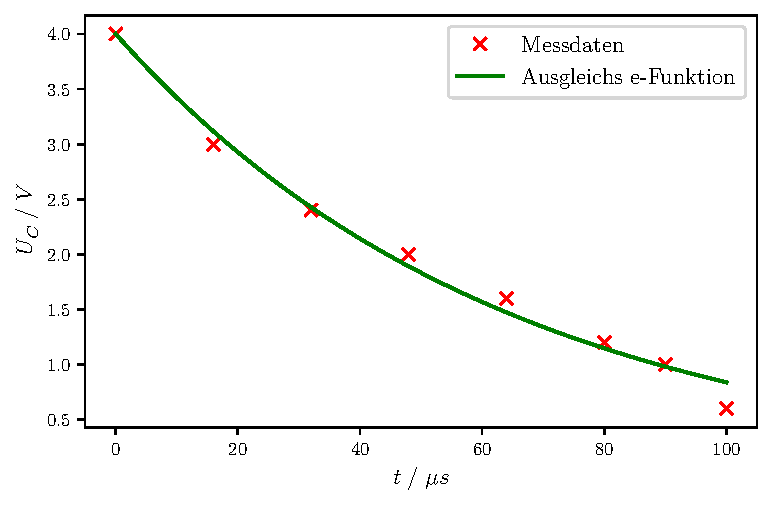
\includegraphics{build/plot_Tex.pdf}
  \caption{Der Abklingvorgang, theoretisch und experimentiell, mit e-Funktion als Fit.}
  \label{fig:plot_abklingdauer}
\end{figure}

Es ergibt sich aus dem Fit an eine e-Funktion mit der Zeitkonstante $k$
\begin{align*}
  k_{exp} = 0.0156 \pm 0.0005 \\
  T_{Abkling,exp} = 64.1 \pm 2.2 \mu s \\
  R_{eff,exp} = 0.000526 \pm 0.000018 \Omega 
\end{align*}
für Abklingdauer und effektiven Widerstand.




\subsection{Bestimmung des Widerstandes beim aperiodischen Grenzfall}
\label{R_ap}

Der experimentiell bestimmte Wert für $R_{ap}$, also der Widerstand, ab dem kein Überschwingen mehr passiert, beträgt $R_{ap,exp} = 4,24 \: k\Omega$. \\
Ein entsprechender Theoriewert dazu lässt sich mit 
\begin{equation*}
  R_{ap,theo} = \sqrt{\frac{4L}{C}} = \sqrt{\frac{4 \cdot 16,87 \cdot 10^{-3}H}{2,060 \cdot 10^{-9}F}} = (5,72 \pm 0,031) \: k\Omega
\end{equation*}
ermitteln.






\subsection{Bestimmung der Frequenzabhängigkeit der Kondensatorspannung}
\label{Kondensatorspannung}

\begin{table}[H]
  \centering
  \caption{Die Kondensatorspannung $U_C$ in Abhängigkeit der Frequenz der Erregerspannung.}
  \begin{tabular}{cc}
    \toprule
    {$f \mathbin{/} \unit{\kilo\hertz}$} &
    {$U_C(t) \mathbin{/} \unit{\volt}$} \\
    \midrule
    20 & 0,75 \\
    22 & 1,05 \\
    24 & 1,35 \\
    26 & 1,65 \\
    28 & 1,50 \\
    30 & 1,10 \\
    32 & 0,80 \\
    34 & 0,55 \\
    36 & 0,50 \\
    38 & 0,40 \\
    40 & 0,35 \\
    42 & 0,30 \\
    44 & 0,25 \\
    46 & 0,20 \\
    48 & 0,16 \\
    50 & 0,19 \\
    52 & 0,15 \\
    54 & 0,13 \\
    56 & 0,12 \\
    58 & 0,11 \\
    60 & 0,10 \\

    \bottomrule
  \end{tabular}
  \label{tab:Tabelle1}
\end{table}


% plot 1, jeweils logarithmisch (in d auch)

\begin{figure}
  \centering
  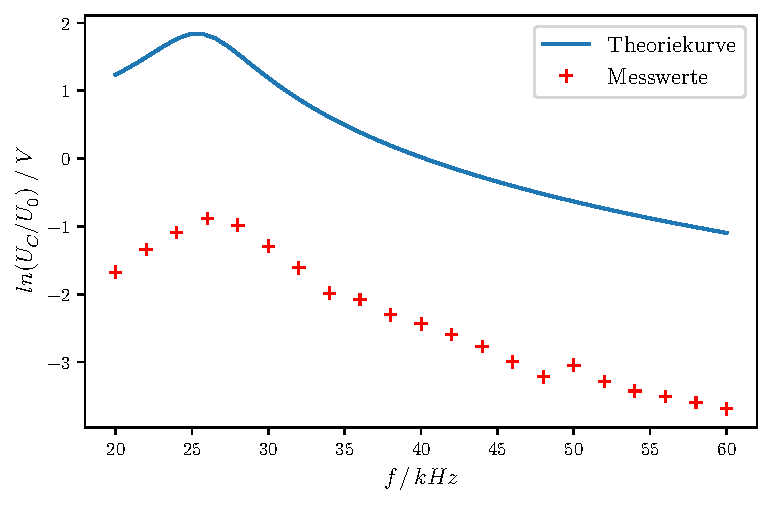
\includegraphics{build/plotc.pdf}
  \caption{Die Frequenzabhängigkeit der Kondensatorspannung $U_C$ halblogarithmisch gegen die Frequenz $f$ aufgetragen.}
  \label{fig:plotc}
\end{figure}



% plot 2, linear, in d auch

\begin{figure}
  \centering
  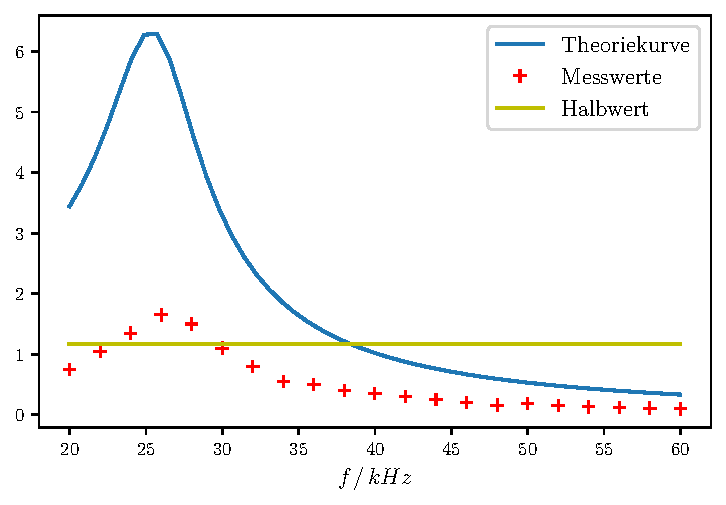
\includegraphics{build/plotc2.pdf}
  \caption{Die Frequenzabhängigkeit der Kondensatorspannung $U_C$ linear gegen die Frequenz $f$ aufgetragen.}
  \label{fig:plotc2}
\end{figure}

Der Theoriewert für die Breite $f_+-f_-$ der Resonanzkurve ergibt sich zu $\frac{R_2}{L} = (6,43 \pm 0.005)\mathrm{kHz}$.\\ 
Mit \autoref{eq:gl11} ergibt sich durch für die experimentiell bestimmte Breite der Resonanzkurve $f_+ - f_- = 6.5 \cdot 10^3 Hz$. \\
Die Frequenzen $f_0$, $f_+$ und $f_-$ betragen $f_0 = 26$ kHz, $f_+ = 29,5$ kHz und $f_- = 23$ kHz. \\
Der experimentielle Wert für die Resonanzüberhöhung $q$ lässt sich also mit Hilfe von $q = \frac{f_0}{f_+ - f_-}$ zu $q = 4$ bestimmen. \\
% Deren theoretischer Wert liegt bei $q = \frac{1}{\omega_0 R C} = $.  weiß nciht genau wie, kommen nur komische werte raus




\subsection{Bestimmung der Frequenzabhängigkeit des Phasenversatzes zwischen $U_{err}$ und $U_{a}$}
\label{Phasenversatz}


\begin{table}[H]
  \centering
  \caption{Der Phasenversatz $\varphi$ in Abhängigkeit der Frequenz der Erregerspannung.}
  \begin{tabular}{cccc}
    \toprule
    {$f \mathbin{/} \unit{\kilo\hertz}$} &
    {$a \mathbin{/} \unit{\micro\second}$} &
    {$b \mathbin{/} \unit{\micro\second}$} &
    {$\varphi \mathbin{/} rad$} \\
    \midrule
    
    20 & 1,0 & 22,0 & 0,286 \\
    22 & 1,5 & 20,0 & 0,471 \\
    24 & 2,5 & 18,0 & 0,872 \\
    26 & 3,5 & 16,5 & 1,332 \\
    28 & 4,5 & 15,0 & 1,884 \\
    30 & 5,0 & 14,0 & 2,244 \\
    32 & 5,5 & 14,0 & 2,468 \\
    34 & 5,5 & 17,5 & 1,975 \\
    36 & 6,0 & 12,0 & 3,142 \\
    38 & 5,0 & 11,0 & 2,856 \\
    40 & 5,0 & 11,0 & 2,856 \\
    42 & 4,5 & 10,5 & 2,693 \\
    44 & 5,0 & 10,0 & 3,142 \\
    46 & 4,0 &  9,0 & 2,793 \\
    48 & 4,0 &  9,0 & 2,793 \\
    50 & 4,5 &  9,5 & 2,976 \\
    52 & 4,0 &  8,0 & 3,142 \\
    54 & 3,5 &  7,5 & 2,932 \\
    56 & 3,5 &  7,5 & 2,932 \\
    58 & 3,5 &  7,5 & 2,932 \\
    60 & 3,0 &  7,0 & 2,693 \\
    
    \bottomrule
  \end{tabular}
  \label{tab:Tabelle2}
\end{table}



\begin{figure}
      \centering
      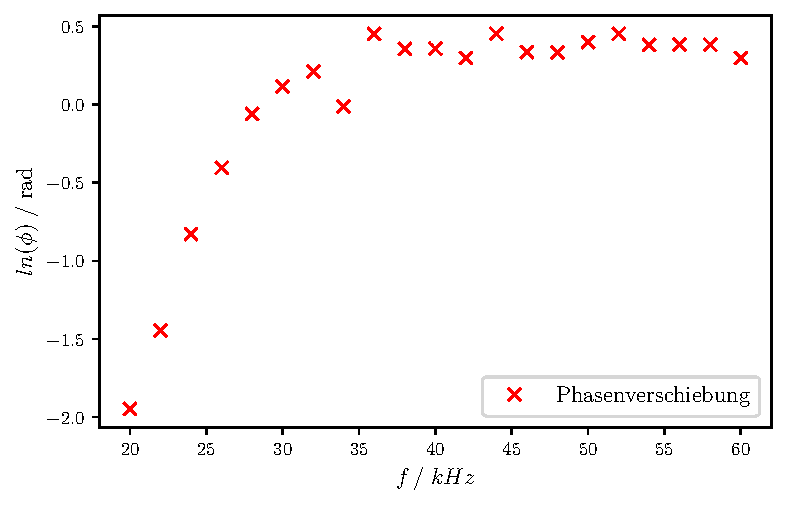
\includegraphics{build/plotd.pdf}
      \caption{Die Phase zwischen $U_C$ und $U_{err}$ in Abhängigkeit der Frequenz von $U_{err}$, halblogarithmisch dargestellt.}
      \label{fig:plotd}
    \end{figure}



    \begin{figure}
      \centering
      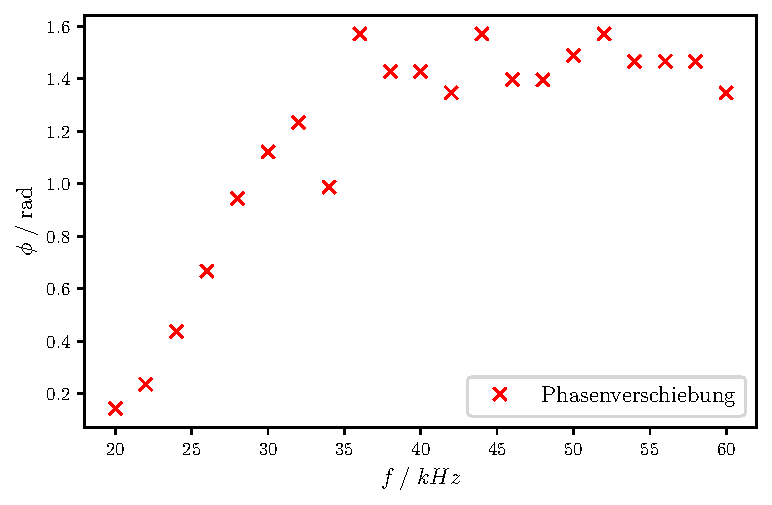
\includegraphics{build/plotd2.pdf}
      \caption{Die Phase zwischen $U_C$ und $U_{err}$ in Abhängigkeit der Frequenz von $U_{err}$, linear dargestellt.}
      \label{fig:plotd2}
    \end{figure}



    